\vspace{30pt}
\section{Part 1}

\subsection{Data organization}
In this subsection relative to Part 1 of the assignment, there is a brief explanation of the initial phase of the assignment itself, which consists of three main steps:
\begin{itemize}
    \item Generation and loading of the file $Group_6.mat$
    \item Data selection
    \item Information extraction from the table
\end{itemize}

After having defined the path to find the session registration data (\texttt{ID\_6\_Session\_1}), the \texttt{make\_group\_mat} function collects and organizes the original data acquired from the MCI, generating the \texttt{Group\_6.mat} file. This file contains the EMG signals, action envelopes, cursor positions, reached targets and calibration information. 
Then, based on the variable "task" value, the corresponding "center-out" or "random" experiment registrations are selected. Here, the focus was associated to the center-out case.
Center-out or random tables are stored in a matrix called "\texttt{D}" and the corresponding targets are stored in a matrix simply called "\texttt{targets}".
Finally, necessary data for the elaborations required for Part 1 are extracted from matrix \texttt{D}.
In the last part, raw EMG signals (expressed in ADC counts) are converted in microvolts. 

\subsection{Part 1 solution}
Part 1 regards the preprocessing of raw EMG signals, allowing to get the activation envelopes starting from raw EMG signals and to compare the results with the ones produced by the MCI system by terms of correlation and temporal difference.
The process follows four steps:
\begin{itemize}
    \item Band-pass filtering
    \item Rectificaton
    \item Low-pass filtering
    \item Normalization
\end{itemize}

\subsubsection{Preprocessing steps for each muscle}
The first initial step allows to transform the raw EMG signals in a measurement of the muscular activation. Initially, a band-pass filter (between 30Hz and 450Hz) is applied to eliminate unwanted low-frequency and high-frequency components. Here, a fourth-order Butterworth filter is projected and the DC offset of each EMG signal is also removed. The filter is applied with the function \texttt{emgFilt}. 
Then, the signals gets rectified with the \texttt{emgRect} function, making its values positive, and filtered with a fourth-order Butterworth low-pass filter at 5Hz to obtain a more regular trend. This result is called activation envelope and it represents the intensity of muscular activation in time. It is stored in \texttt{envOursUV}. Finally, a normalization of these is carried out with respect to the maximum calibration value for each muscle. With this process, values between 0 and 1 are obtained so that the activations of the four muscles are comparable. 
\vspace{20pt}

Here the plotted signals are shown for the four muscles:

\begin{figure}[H]
        \centering
        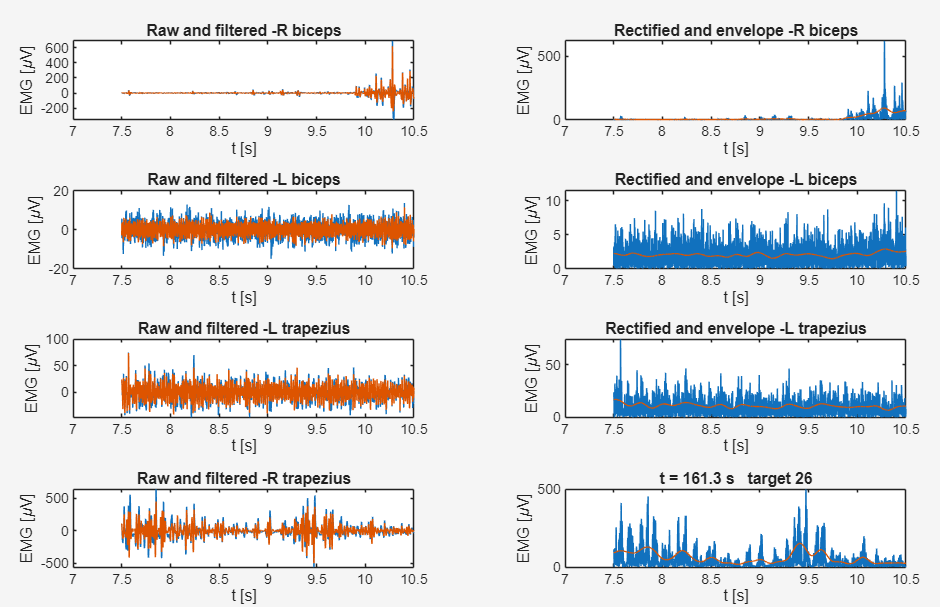
\includegraphics[width=\textwidth]{Images/Our data/raw filtered rectified envelope.png}
        \caption{
        EMG signals processed with the filtering, rectification and DC values elimination processes. \\
        Left images: blue $\rightarrow$ raw signals, red $\rightarrow$ filtered signals. \\
        Right images: blue $\rightarrow$ rectified signals, red $\rightarrow$ envelopes.}
\end{figure}

\vspace{10pt}
\subsubsection{Comparison between the reconstructed and MCI registered envelopes}
Then, in the second part, a quantitative comparison is performed between the reconstructed envelopes \texttt{envOursNorm} and the ones registered by the MCI system \texttt{envMCI}. The correlation matrix between the two envelopes is computed for each muscle to assess how the respective trends are similar. Then, the cross-correlation between signals is computed. With this one, the corresponding delay at the maximum value of the cross-correlation is identified, and it is converted from samples to milliseconds. 

Here, the results are shown from the Command Window:

\begin{figure}[H]
    \centering
    \begin{minipage}{0.30\textwidth}
        \centering
        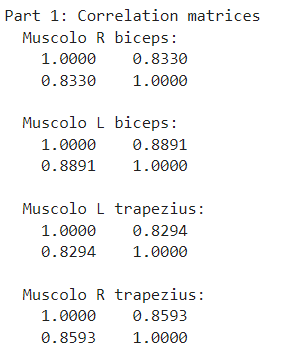
\includegraphics[width=\textwidth]{Images/Our data/part1 correlation matrices.png}
        \caption{Correlation matrices for each muscle}
    \end{minipage}
    \hspace{40pt}
    \begin{minipage}{0.57\textwidth}
        \centering
        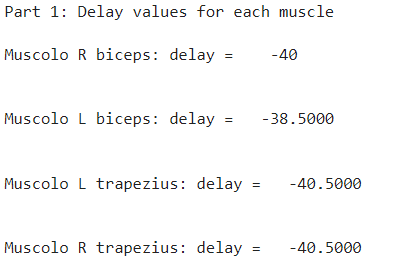
\includegraphics[width=\textwidth]{Images/Our data/part1 delay values for each muscle.png}
        \caption{Delay values from cross-correlation for each muscle}
    \end{minipage}
\end{figure}

\vspace{10pt}
Subsequently, the two envelopes are overlapped, using a time window of 30 seconds, to allow a visual comparison: 

\begin{figure}[H]
        \centering
        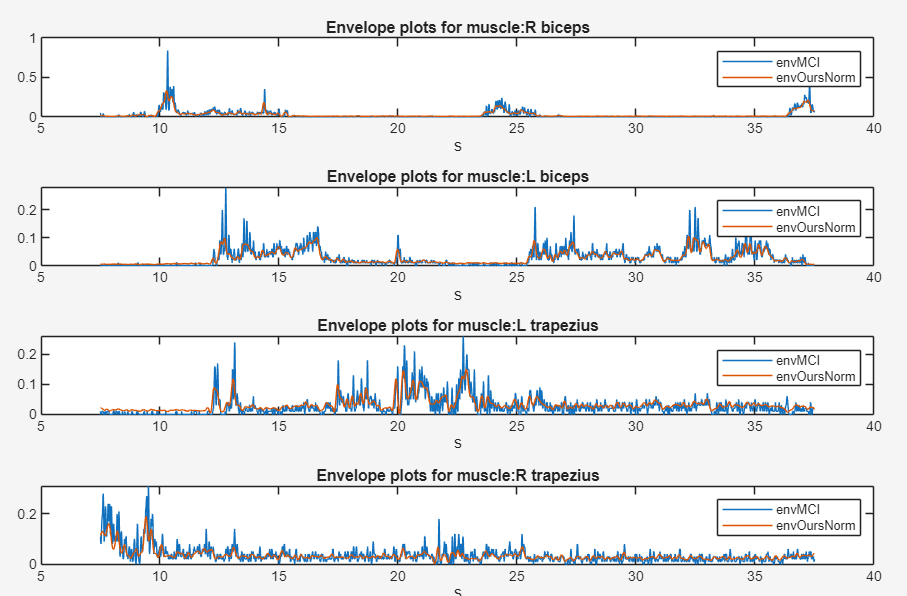
\includegraphics[width=\textwidth]{Images/Our data/envelope plots.png}
        \caption{Overlapped MCI and reconstructed envelopes
        }
\end{figure}

At the end, signals are converted from a sampling frequency of 2000Hz to 100Hz. The downsampling is done only after the filtering and the envelopes computation, since raw EMG signals contain high frequency components that would be lost or altered reducing beforehand the sampling frequency. 

